%% Copyright (c) 2002, 2010 Sam Williams
%% Copyright (c) 2010 Richard M. Stallman
%% Permission is granted to copy, distribute and/or modify this
%% document under the terms of the GNU Free Documentation License,
%% Version 1.3 or any later version published by the Free Software
%% Foundation; with no Invariant Sections, no Front-Cover Texts, and
%% no Back-Cover Texts. A copy of the license is included in the
%% file called ``gfdl.tex''.
\chapter{\ifdefined\eng
St. Ignucius
\fi
\ifdefined\chs
圣·Ignucius
\fi}

\ifdefined\eng
The Maui High Performance Computing Center is located in a single-story building in the dusty red hills just above the town of Kihei. Framed by million-dollar views and the multimillion dollar real estate of the Silversword Golf Course, the center seems like the ultimate scientific boondoggle. Far from the boxy, sterile confines of Tech Square or even the sprawling research metropolises of Argonne, Illinois and Los Alamos, New Mexico, the MHPCC seems like the kind of place where scientists spend more time on their tans than their post-doctoral research projects.
\fi

\ifdefined\chs
茂宜高性能计算中心(Maui High Performance Computing Center)坐落在夏威夷群岛中的茂宜岛上。这是一座单层建筑,建在满是红色火山灰的山岗上,俯瞰茂宜岛的商业中心纪平镇。这个计算中心身在夏威夷,坐拥迷人的山景海风,更有身价千万的房产。这地方好像和高新技术占不上一点边。它跟麻省理工学院技术广场的见楞见角,死气沉沉的气氛完全不同。哪怕跟阿尔贡国家实验室,洛斯阿拉莫斯或者新墨西哥的那些实验室比,茂宜高性能计算中心依旧显得特别。总会难免让人觉得,茂宜计算中心的科学家们每天可能并不怎么关心自己的研究课题,没准他们天天都会把时间花在晒太阳,吹海风上。
\fi

\ifdefined\eng
The image is only half true. Although researchers at the MHPCC do take advantage of the local recreational opportunities, they also take their work seriously. According to \url{Top500.org}, a web site that tracks the most powerful supercomputers in the world, the IBM SP Power3 supercomputer housed within the MHPCC clocks in at 837 billion floating-point operations per second, making it one of 25 most powerful computers in the world. Co-owned and operated by the University of Hawaii and the U.S. Air Force, the machine divides its computer cycles between the number crunching tasks associated with military logistics and high-temperature physics research.
\fi

\ifdefined\chs
不过这个第一感觉可不怎么准确。确实,茂宜计算中心的研究人员的确占尽了地利,也自然会借此休养。不过他们对待工作还是非常认真的。Top500.org 是一个记录全世界超级计算机排名的网站。根据这个网站的资料,茂宜高性能计算中心的IBM SP Power3超级计算机可以每秒完成八千三百七十亿次浮点运算,世界排名前25。这台超级计算机归夏威夷大学和美国空军共同拥有和维护。它主要负责完成军队补给调度计算和高温物理研究。
\fi

\ifdefined\eng
Simply put, the MHPCC is a unique place, a place where the brainy culture of science and engineering and the laid-back culture of the Hawaiian islands coexist in peaceful equilibrium. A slogan on the lab's 2000 web site sums it up: ``Computing in paradise.''
\fi

\ifdefined\chs
简而言之,茂宜计算中心是个非常独特的地方。这地方既有学术研究的文化氛围,又融入了夏威夷上那份慵懒宜人的情调。二者一阴一阳,相得益彰。2000年,他们在自己的官方网站放上了这样一条标语:在天堂之上计算。
\fi

\ifdefined\eng
It's not exactly the kind of place you'd expect to find Richard Stallman, a man who, when taking in the beautiful view of the nearby Maui Channel through the picture windows of a staffer's office, mutters a terse critique: ``Too much sun.'' Still, as an emissary from one computing paradise to another, Stallman has a message to deliver, even if it means subjecting his hacker eyes to painful solar glare.
\fi

\ifdefined\chs
这样一个地方,一般你是见不到理查德·斯托曼身影的。他这次来到这里,站在一位员工办公室的窗口,盯着外面如画的风景,口中却蹦出了一句简单的批评:``阳光太强。''自然,他从计算机界的圣地麻省理工学院来到这里,是有话要讲的。哪怕再强的阳光,刺入这位黑客的双眼,他倒也在所不辞。
\fi

\ifdefined\eng
The conference room is already full by the time I arrive to catch Stallman's speech. The gender breakdown is a little better than at the New York speech, 85\% male, 15\% female, but not by much. About half of the audience members wear khaki pants and logo-encrusted golf shirts. The other half seems to have gone native. Dressed in the gaudy flower-print shirts so popular in this corner of the world, their faces are a deep shade of ochre. The only residual indication of geek status are the gadgets: Nokia cell phones, Palm Pilots, and Sony VAIO laptops.
\fi

\ifdefined\chs
我赶到现场的时候,会议室里早已人满为患,大家都在等待着理查德的演讲。听众中,男女比例倒是比纽约那次的演讲平衡些,不过也没平衡到哪儿去:大约85\%是男性,15\%的女性。有一半的听众,都身穿土黄色的裤子,配上印着商标的高尔夫衬衫。另外一半,则显得更加融入了当地的风俗。身穿宽大的大花T恤,皮肤则已被晒成了褐色。这打扮在夏威夷可是正常装束。唯一能显示他们技术本色的东西,也就只剩下了些小玩意儿了:诺基亚手机,掌上电脑,还有索尼VAIO笔记本。
\fi

\ifdefined\eng
Needless to say, Stallman, who stands in front of the room dressed in plain blue T-shirt, brown polyester slacks, and white socks, sticks out like a sore thumb. The fluorescent lights of the conference room help bring out the unhealthy color of his sun-starved skin.\endnote{RMS: The idea that skin can be ``sun-starved'' or that paleness is ``unhealthy'' is dangerous misinformation; staying out of the sun can't hurt you as long as you have enough Vitamin D. What damages the skin, and can even kill you, is excessive exposure to sunlight.}  His beard and hair are enough to trigger beads of sweat on even the coolest Hawaiian neck. Short of having the words ``mainlander'' tattooed on his forehead, Stallman couldn't look more alien if he tried. [RMS: Is there something bad about looking different from others?]
\fi

\ifdefined\chs
理查德身穿纯蓝色T恤,棕色涤纶休闲裤,白色袜子。不用说,这身行头在当下确实太显眼了。房间中淡淡的花香,倒是让人没太注意理查德缺少阳光滋润的皮肤\endnote{理查德注:所谓``缺少阳光滋润'',或者``越晒太阳越健康''的概念实在是非常误导人。在太阳底下不被晒伤的前提是你需要有足够的维生素D。而过度在阳光下暴晒,不仅可能损害皮肤,甚至可能要人命。}。不过他一头长发和络腮胡须却依旧能引人注目。外人一看,就知道他不是本地人。他就差在脑门上贴个标签,写着:``美国本土人士。''[RMS:把自己打扮得和别人不一样有什么不对吗?]
\fi

\ifdefined\eng
As Stallman putters around the front of the room, a few audience members wearing T-shirts with the logo of the Maui FreeBSD Users Group (MFUG) race to set up camera and audio equipment. FreeBSD, a free software offshoot of the Berkeley Software Distribution, the venerable 1970s academic version of Unix, is technically a competitor to the GNU/Linux operating system. Still, in the hacking world, Stallman speeches are documented with a fervor reminiscent of the Grateful Dead and its legendary army of amateur archivists. As the local free software heads, it's up to the MFUG members to make sure fellow programmers in Hamburg, Mumbai, and Novosibirsk don't miss out on the latest pearls of RMS wisdom.
\fi

\ifdefined\chs
演讲开始前,理查德自己在会议室前面闲逛。旁边几个人鼓捣着录像录音器材。这些人都身穿``茂宜FreeBSD用户组''(Maui FreeBSD User Group,MFUG)的T恤。所谓FreeBSD,是一款从伯克利软件发行版的UNIX系统分支而来的操作系统。而伯克利版UNIX则是七十年代由加州大学伯克利分校开发的一个UNIX分支。说起来,FreeBSD倒还是GNU/Linux的一个竞争对手。在黑客的世界里,理查德的演讲总会被记录拍摄下来,留做档案。作为当地的著名自由软件组织,茂宜FreeBSD用户组可不能让同行失望。他们也要录音录像,让远在德国汉堡,印度孟买,俄罗斯新西伯利亚等世界各地的黑客们,都能听到RMS的箴言。
\fi

\ifdefined\eng
The analogy to the Grateful Dead is apt. Often, when describing the business opportunities inherent within the free software model, Stallman has held up the Grateful Dead as an example. In refusing to restrict fans' ability to record live concerts, the Grateful Dead became more than a rock group. They became the center of a tribal community dedicated to Grateful Dead music. Over time, that tribal community became so large and so devoted that the band shunned record contracts and supported itself solely through musical tours and live appearances. In 1994, the band's last year as a touring act, the Grateful Dead drew \$52 million in gate receipts alone.\endnote{See ``Grateful Dead Time Capsule: 1985-1995 North American Tour Grosses,'' \url{http://www.dead101.com/1197.htm}.}
\fi

\ifdefined\chs
理查德的这些演讲记录,就像是感恩而死乐队(Grateful Dead)的现场演出一样,都是被追捧者现场录下,私下传递。把理查德和感恩而死乐队做类比,可是有说头的。每当理查德描述自由软件的商业盈利模式的时候,他都会提起感恩而死乐队。这个乐队当年允许粉丝们在现场录音录像,这就令它不仅是一个简单的摇滚乐队。它俨然成了感恩而死音乐部落的中心。逐渐地,这个部落越来越大,令感恩而死乐队拒绝了各种唱片公司的合约,完全靠巡回演出,就可以撑起整个乐队的开支。在1994年,这支乐队的最后一次演出仅门票收入就高达五千两百万美元\endnote{参见《1985至1995北美演出收入排行榜》 http://www.dead101.com/1197.htm}。
\fi

\ifdefined\eng
While few software companies have been able to match that success, the tribal aspect of the free software community is one reason many in the latter half of the 1990s started to accept the notion that publishing software source code might be a good thing. Hoping to build their own loyal followings, companies such as IBM, Sun Microsystems, and Hewlett Packard have come to accept the letter, if not the spirit, of the Stallman free software message. Describing the GPL as the information-technology industry's \textit{Magna Carta}, ZDNet software columnist Evan Leibovitch sees the growing affection for all things GNU as more than just a trend. ``This societal shift is letting users take back control of their futures,'' Leibovitch writes. ``Just as the \textit{Magna Carta} gave rights to British subjects, the GPL enforces consumer rights and freedoms on behalf of the users of computer software.''\endnote{See Evan Leibovitch, ``Who's Afraid of Big Bad Wolves,'' \textit{ZDNet Tech Update} (December 15, 2000), \url{http://www.zdnet.com/news/whos-afraid-of-the-big-bad-wolves/298394}.}
\fi

\ifdefined\chs
当然,还没有哪个软件公司的成就可以媲美感恩而死乐队。不过,自由软件社区的这个部落越来越大,在九十年代后期,大家也逐渐开始认为分享发布软件的源代码没准是个好事。各大公司纷纷出马,企图建立起各自的忠实粉丝群。这其中就包括IBM,Sun,惠普等。它们也许并没有打心眼里接受自由软件的看法,但他们的行为却是在响应理查德的号召。ZDNet的软件专栏作家埃文·列伊博维奇(Evan Leibovitch)把GPL(GNU通用公共许可证,理查德创立的一种自由软件许可证,用于规定软件作者授予软件用户的各种权利)描述为信息时代的大宪章。他认为,人们对于GNU的拥护持续高涨,并非单纯地跟风。他曾写道:``这个趋势让用户可以重新掌控自己的命运。就好像当年《大宪章》给了英国人民权利。GPL让消费者作为计算机软件用户有了自己的权利和自由\endnote{参见埃文·列伊博维奇(Evan Leibovitch)在文章《谁会害怕大灰狼》,2000年12月15日,ZDNet Tech Update. http://www.zdnet.com/news/whos-afraid-of-the-big-bad-wolves/298394}。''
\fi

\ifdefined\eng
The tribal aspect of the free software community also helps explain why 40-odd programmers, who might otherwise be working on physics projects or surfing the Web for windsurfing buoy reports, have packed into a conference room to hear Stallman speak.
\fi

\ifdefined\chs
自由软件社区的这种部落文化也解释了为什么今天这四十来位古怪的程序员们,可以暂时不管各自的工作,也不去上网冲浪,而宁愿能挤在这个会议室里,听理查德的讲座。
\fi

\ifdefined\eng
Unlike the New York speech, Stallman gets no introduction. He also offers no self-introduction. When the FreeBSD people finally get their equipment up and running, Stallman simply steps forward, starts speaking, and steamrolls over every other voice in the room.
\fi

\ifdefined\chs
和那次在纽约的讲座不一样,这次没有人为他做开场白,理查德自己也没做自我介绍。FreeBSD用户组的人把设备一架好,理查德就自己踏上前来,开始演讲,声音一下盖过了台下的私语。
\fi

\ifdefined\eng
``Most of the time when people consider the question of what rules society should have for using software, the people considering it are from software companies, and they consider the question from a self-serving perspective,'' says Stallman, opening his speech. ``What rules can we impose on everybody else so they have to pay us lots of money? I had the good fortune in the 1970s to be part of a community of programmers who shared software. And because of this I always like to look at the same issue from a different direction to ask: what kind of rules make possible a good society that is good for the people who are in it? And therefore I reach completely different answers.''
\fi

\ifdefined\chs
``一个社会该给软件的使用设立何种规则?每当想到这个问题,大多数人总是站在软件公司的立场思考。他们的想法往往像是在自我圆场。''理查德开门见山:``他们想:我们如何设立规则,才能让大家多给我们钱呢?我很幸运,在七十年代,曾加入了一个大家庭,在那里面,大家都会互相分享软件。正因如此,我总会从另外一个角度去思考这个问题:我们应该如何设立规则,才能帮助我们构建一个更好的社会,一个可以让每个人都受益的社会?也正因如此,我得到了完全不一样的答案。''
\fi

\ifdefined\eng
Once again, Stallman quickly segues into the parable of the Xerox laser printer, taking a moment to deliver the same dramatic finger-pointing gestures to the crowd. He also devotes a minute or two to the GNU/Linux name.
\fi

\ifdefined\chs
理查德又一次提起了施乐打印机事件,形式和以前很像,同样是讲到最后,手指指向听众,口中说着:``也许就会背叛你!''之后,他又花了一两分钟,来解释GNU/Linux的名字问题。
\fi

\ifdefined\eng
``Some people say to me, `Why make such a fuss about getting credit for this system? After all, the important thing is the job is done, not whether you get recognition for it.' Well, this would be wise advice if it were true. But the job wasn't to build an operating system; the job is to spread freedom to the users of computers. And to do that we have to make it possible to do everything with computers in freedom.''\endnote{For narrative purposes, I have hesitated to go in-depth when describing Stallman's full definition of software ``freedom.'' The GNU Project web site lists four fundamental components:

\begin{itemize}
  \item The freedom to run the program as you wish, for any purpose (freedom 0).
  \item The freedom to study the program's source code, and change it so that the program does what you wish (freedom 1).
  \item The freedom to redistribute copies of the program so you can help your neighbor (freedom 2).
  \item The freedom to distribute copies of your modified versions, so that the whole community can benefit from them (freedom 3).
\end{itemize}

For more information, please visit ``The Free Software Definition'' at \url{http://www.gnu.org/philosophy/free-sw.html}.}
\fi

\ifdefined\chs
``有些人会和我说:`你为什么要花这么多精力去在乎人们叫它什么?为什么非要在乎这种名利上的事?如今任务已经做完了,你何必非要在乎人们有没有注意到GNU呢?'这个……如果这话描述的是事实,那我确实同意这话的观点。可现实是:我们的任务并没有完成。我们的任务不是要创造一套操作系统;我们的任务是要给计算机用户自由。要完成这个任务,我们必须要尽一切努力,让用户可以自由地使用计算机和软件\endnote{...........}。''
\fi

\ifdefined\eng
Adds Stallman, ``There's a lot more work to do.''
\fi

\ifdefined\chs
理查德最后说:``我们要走的路还很长。''
\fi

\ifdefined\eng
For some in the audience, this is old material. For others, it's a little arcane. When a member of the golf-shirt contingent starts dozing off, Stallman stops the speech and asks somebody to wake the person up.
\fi

\ifdefined\chs
对于一些听众来说,理查德的这些话是老生长谈了。对于其他人来说,这些话则有点令人不可思议了。旁边那个身穿高尔夫T恤的听众已经开始打盹了,理查德停下来,让旁边的人把这位叫醒。
\fi

\ifdefined\eng
``Somebody once said my voice was so soothing, he asked if I was some kind of healer,'' says Stallman, drawing a quick laugh from the crowd. ``I guess that probably means I can help you drift gently into a blissful, relaxing sleep. And some of you might need that. I guess I shouldn't object if you do. If you need to sleep, by all means do.''
\fi

\ifdefined\chs
``曾经有个人,说我的声音特别像安慰剂,他问我是不是做过催眠师之类的工作。''理查德说着,下面一阵笑声。在笑声中他接着说:``我想这意味着我可以帮你们快速进入梦乡。可能你们之中有些人正想要这样。我觉得我确实也不该打搅你们,你要是真想睡觉,尽管睡吧。''
\fi

\ifdefined\eng
The speech ends with a brief discussion of software patents, a growing issue of concern both within the software industry and within the free software community. Like Napster, software patents reflect the awkward nature of applying laws and concepts written for the physical world to the frictionless universe of information technology.
\fi

\ifdefined\chs
演讲最后,斯托曼简要地探讨了软件专利的问题。这个问题逐渐在软件业和自由软件社区中受到关注。专利的概念和想法本是为现实的物理世界准备。可把它用在信息世界中,就越来越显得古怪了。
\fi

\ifdefined\eng
Copyright law and patent law work differently, and have totally different effects in the software field.  The copyright on a program controls the copying and adaptation of that program's code, and it belongs to the program's developer.  But copyright does not cover ideas. In other words, a developer is free, under copyright, to implement in his own code features and commands he has seen in existing programs.  Those aspects are ideas, not expression, and thus outside the scope of copyright law.
\fi

\ifdefined\chs
版权和专利是两个不同的概念,也有着完全不同的目的。对于软件来说,版权法用来约束拷贝或修改软件代码的行为。一个程序的版权是归开发者所有。但是版权不能保护作者的想法。换句话说,开发者可以克隆一个已经存在的软件,只要他不去复制别人的代码,就不会涉及到版权问题。因为这是在重现别人的想法,所以这在版权法的作用范围之外。
\fi

\ifdefined\eng
It is likewise lawful -- though hard work -- to decode how a binary program works, and then implement the same ideas and algorithms in different code.  This practice is known as ``reverse engineering.''
\fi

\ifdefined\chs
如果开发者直接阅读软件的机器码,尽管会比较费事费力,但这依旧是合法的。同理,开发者也可以通过阅读软件的机器码,再自己独立实现一个类似的软件。这个做法通常被称作``逆向工程''。
\fi

\ifdefined\eng
Software patents work differently. According to the U.S. Patent Office, companies and individuals can obtain patents for computing ideas that are innovative (or, at least, unknown to the Patent Office). In theory, this allows the patent-holder to trade off disclosure of the technique for a specific monopoly lasting a minimum of 20 years after the patent filing. In practice, the disclosure is of limited value to the public, since the operation of the program is often self-evident, and could in any case be determined by reverse engineering. Unlike copyright, a patent gives its holder the power to forbid the independent development of software programs which use the patented idea.
\fi

\ifdefined\chs
可软件专利就不同了。按照美国专利局的说法,个人或公司的计算方面的创新想法,可以获得专利(准确说,所谓创新想法,也就是专利局没听说过的想法)。理论上讲,专利拥有者需要公开自己的创新想法,由此可以垄断这个创造至少二十年,计时从专利提交起开始。但是实际上,公开专利的创新想法并不能怎么让公众受益。因为程序的想法往往是不言自明的。或者可以通过逆向工程获得。而专利法和版权法不同,它禁止任何人实现专利上描述的想法,哪怕开发者是独立开发的。
\fi

\ifdefined\eng
In the software industry, where 20 years can cover the entire life cycle of a marketplace, patents take on a strategic weight. Where companies such as Microsoft and Apple once battled over copyright and the ``look and feel'' of various technologies, today's Internet companies use patents as a way to stake out individual applications and business models, the most notorious example being Amazon.com's 2000 attempt to patent the company's ``one-click'' online shopping process. For most companies, however, software patents have become a defensive tool, with cross-licensing deals balancing one set of corporate patents against another in a tense form of corporate detente. Still, in a few notable cases of computer encryption and graphic imaging algorithms, software vendors have successfully stifled rival developments.  For instance, some font-rendering features are missing from free software because of patent threats from Apple.
\fi

\ifdefined\chs
在软件世界里,二十年的时间可能覆盖了一个市场的整个生命周期。这样,专利就成了一种策略。当年,微软和苹果这些大公司为版权打得不可开交。而如今那些互联网企业,则使用专利来为自己开路,赶走竞争对手和新人。这里有个著名的案例。2000年,亚马逊购物曾试图为它的``一键购买''功能注册专利。简单说,这个功能就是允许用户事先存储好个人信息——比如信用卡信息,收件人地址等——然后在购买商品的时候,只需要按一个按钮,就可以下单,不必再跳转到其他页面填写地址,付款等信息。对于大多数公司来说,软件专利更像是一种防卫措施。几个公司可能会合作共有一系列专利,用来阻止另外一个联盟的专利。尽管如此,还是有不少领域被软件专利占满,阻碍了各种可能的竞争对手。比如图像处理领域,加密领域等等。比较实际的例子是,一些字体渲染算法,不会出现在自由软件中,因为苹果公司持有这些算法的专利。
\fi

\ifdefined\eng
For Stallman, the software-patent issue dramatizes the need for eternal hacker vigilance. It also underlines the importance of stressing the political benefits of free software programs over the competitive benefits. Stallman says competitive performance and price, two areas where free software operating systems such as GNU/Linux and FreeBSD already hold a distinct advantage over their proprietary counterparts, are side issues compared to the large issues of user and developer freedom.
\fi

\ifdefined\chs
对于理查德来说,软件专利更督促着黑客要时刻警觉,而且还凭添了几分戏剧色彩。也恰恰是软件专利,让自由软件一直强调的政治策略再次得以重申。即,用户的自由比其他更重要。理查德说,高性能,低价格等特性的确是GNU/Linux,FreeBSD等这些自由软件的优势。但是除了性能,价格这些东西以外,还有更重大的问题,那就是用户和开发者的自由。
\fi

\ifdefined\eng
This position is controversial within the community: open source advocates emphasize the utilitarian advantages of free software over the political advantages. Rather than stress the political significance of free software programs, open source advocates have chosen to stress the engineering integrity of the hacker development model. Citing the power of peer review, the open source argument paints programs such as GNU/Linux or FreeBSD as better built, better inspected and, by extension, more trustworthy to the average user.
\fi

\ifdefined\chs
这个观点在圈子里也饱受争议:开源的支持者们喜欢强调自由软件的实用性,会避免探讨用户自由之类的问题。他们可能不会强调这些,转而强调黑客开发的工程模型。强调同行互相审校的重要性。他们认为,GNU/Linux或FreeBSD的开发模式可以创造出更好,更强大,更值得信赖的软件。
\fi

\ifdefined\eng
That's not to say the term ``open source'' doesn't have its political implications. For open source advocates, the term open source serves two purposes. First, it eliminates the confusion associated with the word ``free,'' a word many businesses interpret as meaning ``zero cost.'' Second, it allows companies to examine the free software phenomenon on a technological, rather than ethical, basis. Eric Raymond, cofounder of the Open Source Initiative and one of the leading hackers to endorse the term, explained his refusal to follow Stallman's political path in a 1999 essay, titled ``Shut Up and Show Them the Code'':
\fi

\ifdefined\chs
但是,``开源''一词也并非意味着没有任何政治诉求。对于开源支持者来说,开源有着两重含义。第一,它避免了在英文中使用Free一词。自由软件的英文是Free Software,因为Free在英文中既有自由的意思,也有免费的意项,所以难免会产生歧义。很多商业公司会觉得自由软件等于免费软件。使用``开源''一词的动机之一,就是希望消除这种歧义。第二,它让商业公司可以从技术角度去审视自由软件,而不必在道义过多解读。艾瑞克·雷蒙德(Eric Raymond)是开放源代码促进会(Open Source Initiative,缩写:OSI)的联合创始人之一,也是支持使用``开源''一词的著名黑客。他曾在1999年发表了一篇文章,用以表明他拒绝接受理查德的政治路线。文章标题是《少说话,秀代码》(Shut Up and Show Them the Code):
\fi

\ifdefined\eng
\begin{quote}
RMS's rhetoric is very seductive to the kind of people we are. We hackers are thinkers and idealists who readily resonate with appeals to ``principle'' and ``freedom'' and ``rights.'' Even when we disagree with bits of his program, we want RMS's rhetorical style to work; we think it ought to work; we tend to be puzzled and disbelieving when it fails on the 95\% of people who aren't wired like we are.\endnote{See Eric Raymond, ``Shut Up and Show Them the Code,'' online essay, (June 28, 1999), \url{http://www.catb.org/~esr/writings/shut-up-and-show-them.html}.}
\end{quote}
\fi

\ifdefined\chs
RMS[即,理查德·M·斯托曼的缩写]的用词对于我们这样的人来说很有吸引力。我们黑客都是思考者,都是理想主义者。我们都时刻准备着响应支持``自由'',``原则''和``权利''的号召。哪怕我们有时候会与理查德的一些意见不同,但我们依旧希望他的做法能有效。我们觉得他的言辞应该有效。可是,我们看到世界上另外95\%的人和我们不一样,理查德的言论对他们无效。面对这些,我们开始迷惑,甚至怀疑。
\fi

\ifdefined\eng
Included among that 95\%, Raymond writes, are the bulk of business managers, investors, and nonhacker computer users who, through sheer weight of numbers, tend to decide the overall direction of the commercial software marketplace. Without a way to win these people over, Raymond argues, programmers are doomed to pursue their ideology on the periphery of society:
\fi

\ifdefined\chs
雷蒙德写道,那另外95\%的人中,包括很多公司经理,投资人,还有普通的计算机用户,他们不是黑客,他们会倾向于跟从专有商业软件的大市场。雷蒙德认为,如果不能赢得这些人的支持,黑客们将只能游离于主流之外,去追随自己的理想。
\fi

\ifdefined\eng
\begin{quote}
When RMS insists that we talk about ``computer users' rights,'' he's issuing a dangerously attractive invitation to us to repeat old failures. It's one we should reject -- not because his principles are wrong, but because that kind of language, applied to software, simply does not persuade anybody but us. In fact, it confuses and repels most people outside our culture.\endnote{\textit{Ibid.}}
\end{quote}
\fi

\ifdefined\chs
\begin{quote}
理查德向我们谈论起``计算机用户权利''的时候,他向我们发出了一份吸引人却危险的邀请函,引导着我们重犯旧错。我们应该拒绝它——不是因为它的原则是错的,而是因为那样的词汇用在软件上,只能说服我们自己,而不能说服别人。事实是,它把大多数圈外人都拒之千里\endnote{\textit{同上。}}。
\end{quote}
\fi

\ifdefined\eng
Stallman, however, rejects Raymond's premises:
\fi

\ifdefined\chs
但是,理查德却反对雷蒙德的说法:
\fi

\ifdefined\eng
\begin{quote}
Raymond's attempt to explain our failure is misleading because we have not failed.  Our goal is large, and we have a long way to go, but we have also come a long way.

Raymond's pessimistic assertion about the values of non-hackers is an exaggeration.  Many non-hackers are more concerned with the political issues we focus on than with the technical advantages that open source emphasizes.  This often includes political leaders too, though not in all countries.

It was the ethical ideals of free software, not ``better software,'' which persuaded the presidents of Ecuador and Brazil to move government agencies to free software.  They are not geeks, but they understand freedom.
\end{quote}
\fi

\ifdefined\chs
\begin{quote}
雷蒙德对我们失败的解释非常有误导性。因为我们压根都没有失败呢。我们为自己设定的目标很远,我们还有多长的路要走。可是要知道,我们已经走过了很多路,克服了很多困难。

雷蒙德关于大众的悲观判断是夸大其辞。很多人不是黑客,但是却同样关注我们强调的政治问题,他们也认为自由的问题比开源所强调的技术优势要重要。这些人之中,甚至会有一些政治领导人。

厄瓜多尔和巴西的政府恰恰就是因为考虑到道义问题,而不是技术问题,才让政府计算机使用自由软件。他们可不是黑客,但他们也理解其中的自由。

\end{quote}
\fi

\ifdefined\eng
But the principal flaw in the open source argument, according to Stallman, is that it leads to weaker conclusions.  It convinces many users to run some programs which are free, but does not offer them any reason to migrate entirely to free software.  This partially gives them freedom, but does not teach them to recognize it and value it as such, so they remain likely to let it drop and lose it.  For instance, what happens when the improvement of free software is blocked by a patent?
\fi

\ifdefined\chs
对于理查德来说,开源的重大问题,在于得出了过于宽松的结论。它可以说服用户去使用自由软件,但却无法提供更多的理由,让用户完全放弃专有软件。这只能给用户部分自由,却不能教会用户去珍视自由。最终,用户还是很可能继续掉入专有软件的陷阱,本来的那些自由也从此丢失。举个例子,如果因为专利问题,让某个自由软件无法添加某项功能,用户该做何选择?
\fi

\ifdefined\eng
Most open source advocates are equally, if not more, vociferous as Stallman when it comes to opposing software patents.  So too are most proprietary software developers, since patents threaten their projects too.  However, pointing to software patents' tendency to put areas of software functionality off limits, Stallman contrasts what the free software idea and the open source idea imply about such cases.
\fi

\ifdefined\chs
大多数开源支持者们也会和理查德一样,极力反对软件专利。甚至很多专有软件的开发者也一样反对软件专利,因为软件专利也同样威胁着他们的项目。然而,理查德指出,软件专利会阻止人们实现某些功能。这里,开源和自由软件在理念上的分歧就显现出来了:
\fi

\ifdefined\eng
``It's not because we don't have the talent to make better software,'' says Stallman. ``It's because we don't have the right. Somebody has prohibited us from serving the public. So what's going to happen when users encounter these gaps in free software? Well, if they have been persuaded by the open source movement that these freedoms are good because they lead to more-powerful reliable software, they're likely to say, `You didn't deliver what you promised. This software's not more powerful. It's missing this feature. You lied to me.' But if they have come to agree with the free software movement, that the freedom is important in itself, then they will say, `How dare those people stop me from having this feature and my freedom too.' And with that kind of response, we may survive the hits that we're going to take as these patents explode.''
\fi

\ifdefined\chs
``这个时候,我们如果做不出更好的软件,并不是能力不足。而是因为有人利用专利,故意阻止我们为公众服务。倘若一位用户使用的自由软件中,由于某项专利,而缺少一个功能,用户会作何反应呢?如果当初这些用户是被开源软件的理念说服而使用这个自由软件,那么他们当初学到的是:给予用户自由是为了创造更强大可靠的软件。这时候,遇到软件缺少功能,他们会说,`你们没能给我一个强大可靠的软件,它少了这个功能,你们骗了我。'相反,如果这个用户是因为认同自由软件的价值观,而使用自由软件的话,那么他们会说:`那些专利竟然阻止了这个功能的实现,剥夺了我的自由。'只有用户认同自由软件的价值观,那么面对大量的软件专利,我们才可能幸存。''
\fi

\ifdefined\eng
Watching Stallman deliver his political message in person, it is hard to see anything confusing or repellent. Stallman's appearance may seem off-putting, but his message is logical. When an audience member asks if, in shunning proprietary software, free software proponents lose the ability to keep up with the latest technological advancements, Stallman answers the question in terms of his own personal beliefs. ``I think that freedom is more important than mere technical advance,'' he says. ``I would always choose a less advanced free program rather than a more advanced nonfree program, because I won't give up my freedom for something like that [advance]. My rule is, if I can't share it with you, I won't take it.''
\fi

\ifdefined\chs
看着理查德阐述自己的政治诉求,并不会让人迷惑或厌恶。他衣着朴素,说起话来有理有据,逻辑清晰。听众中一位提问:如果完全避免使用专有软件,可能无法用到最新的技术,该怎么办?理查德引述自己的信念,回答了这个问题:``我觉得自由本身比任何新近技术都重要。如果面前有一个先进的专有软件,和一个技术落后的自由软件,那么我宁愿选择后者。因为无论如何,我都不会靠出卖自由,而换取更新的技术。我的原则是,如果我不能和你分享这个软件,我就不会使用它。''
\fi

\ifdefined\eng
In the minds of those who assume ethics means religion, such answers reinforce the quasi-religious nature of the Stallman message. However, unlike a Jew keeping kosher or a Mormon refusing to drink alcohol, Stallman is not obeying a commandment, but simply refusing to cede his freedom.  His speech explains the practical requisites for doing so: a proprietary program takes away your freedom, so if you want freedom, you need to reject the program.
\fi

\ifdefined\chs
有些人可能会把道义问题和宗教信仰联系起来。理查德的这个回答则更可能给人一种宗教信仰的感觉。不过,理查德的行为不同于犹太人只吃洁食的行为,也不同于摩门教徒不喝酒。理查德并不是要守着清规戒律,他只是不想牺牲自己的自由。他的演讲解释了他的思路:专有软件会剥夺你的自由,如果你想要自由,你就要拒绝使用专有软件。
\fi

\ifdefined\eng
Stallman paints his decision to use free software in place of proprietary in the color of a personal belief he hopes others will come to share. As software evangelists go, Stallman avoids forcing those beliefs down listeners' throats. Then again, a listener rarely leaves a Stallman speech not knowing where the true path to software righteousness lies.
\fi

\ifdefined\chs
理查德仅仅使用自由软件,拒绝任何专有软件。他把这描述为个人信仰,并且希望把这份信仰与大家一同分享。但他不会强迫别人认同自己。大多数听众,在听过理查德的演讲之后,都会明白理查德所说的正确的软件之路。
\fi

\ifdefined\eng
As if to drive home this message, Stallman punctuates his speech with an unusual ritual. Pulling a black robe out of a plastic grocery bag, Stallman puts it on.  Then he pulls out a reflective brown computer disk and places it on his head. The crowd lets out a startled laugh.
\fi

\ifdefined\chs
演讲最后,像个总结一样,理查德开始了一个不太寻常的仪式。他从一个百货商店的塑料购物袋里,掏出了一条黑色长袍。他把长袍打开,套在了身上。接着,又从袋子里拿出来了一个圆形的老式计算机硬盘碟片,把它戴在头上。这碟片一戴上,就像极了基督教圣徒头顶的光环。看到这身扮相,人群中传来了一阵笑声。
\fi

\ifdefined\eng
``I am St. IGNUcius of the Church of Emacs,'' says Stallman, raising his right hand in mock-blessing. ``I bless your computer, my child.''
\fi

\ifdefined\chs
``我是圣·IGNUcius\endnote{圣·IGNUcius(St. IGNUcius),名字中包含了GNU三个字母。这个名字可能来自基督教圣人伊格那丢(St. Ignatius)。伊格那丢被罗马皇帝投入野兽笼中而死。理查德的圣·IGNUcius本身并没有任何宗教意义(理查德本人是无神论者),仅仅出于玩笑心理,起了这么个名字:既能在字面上和基督教圣徒有些类似,又能把GNU三个字母放进名字里。},来自Emacs教堂。''理查德举起右手,好似在为众人祈福:``我保佑你的计算机,孩子们。''
\fi

\ifdefined\eng
\begin{figure}[ht] \centering
  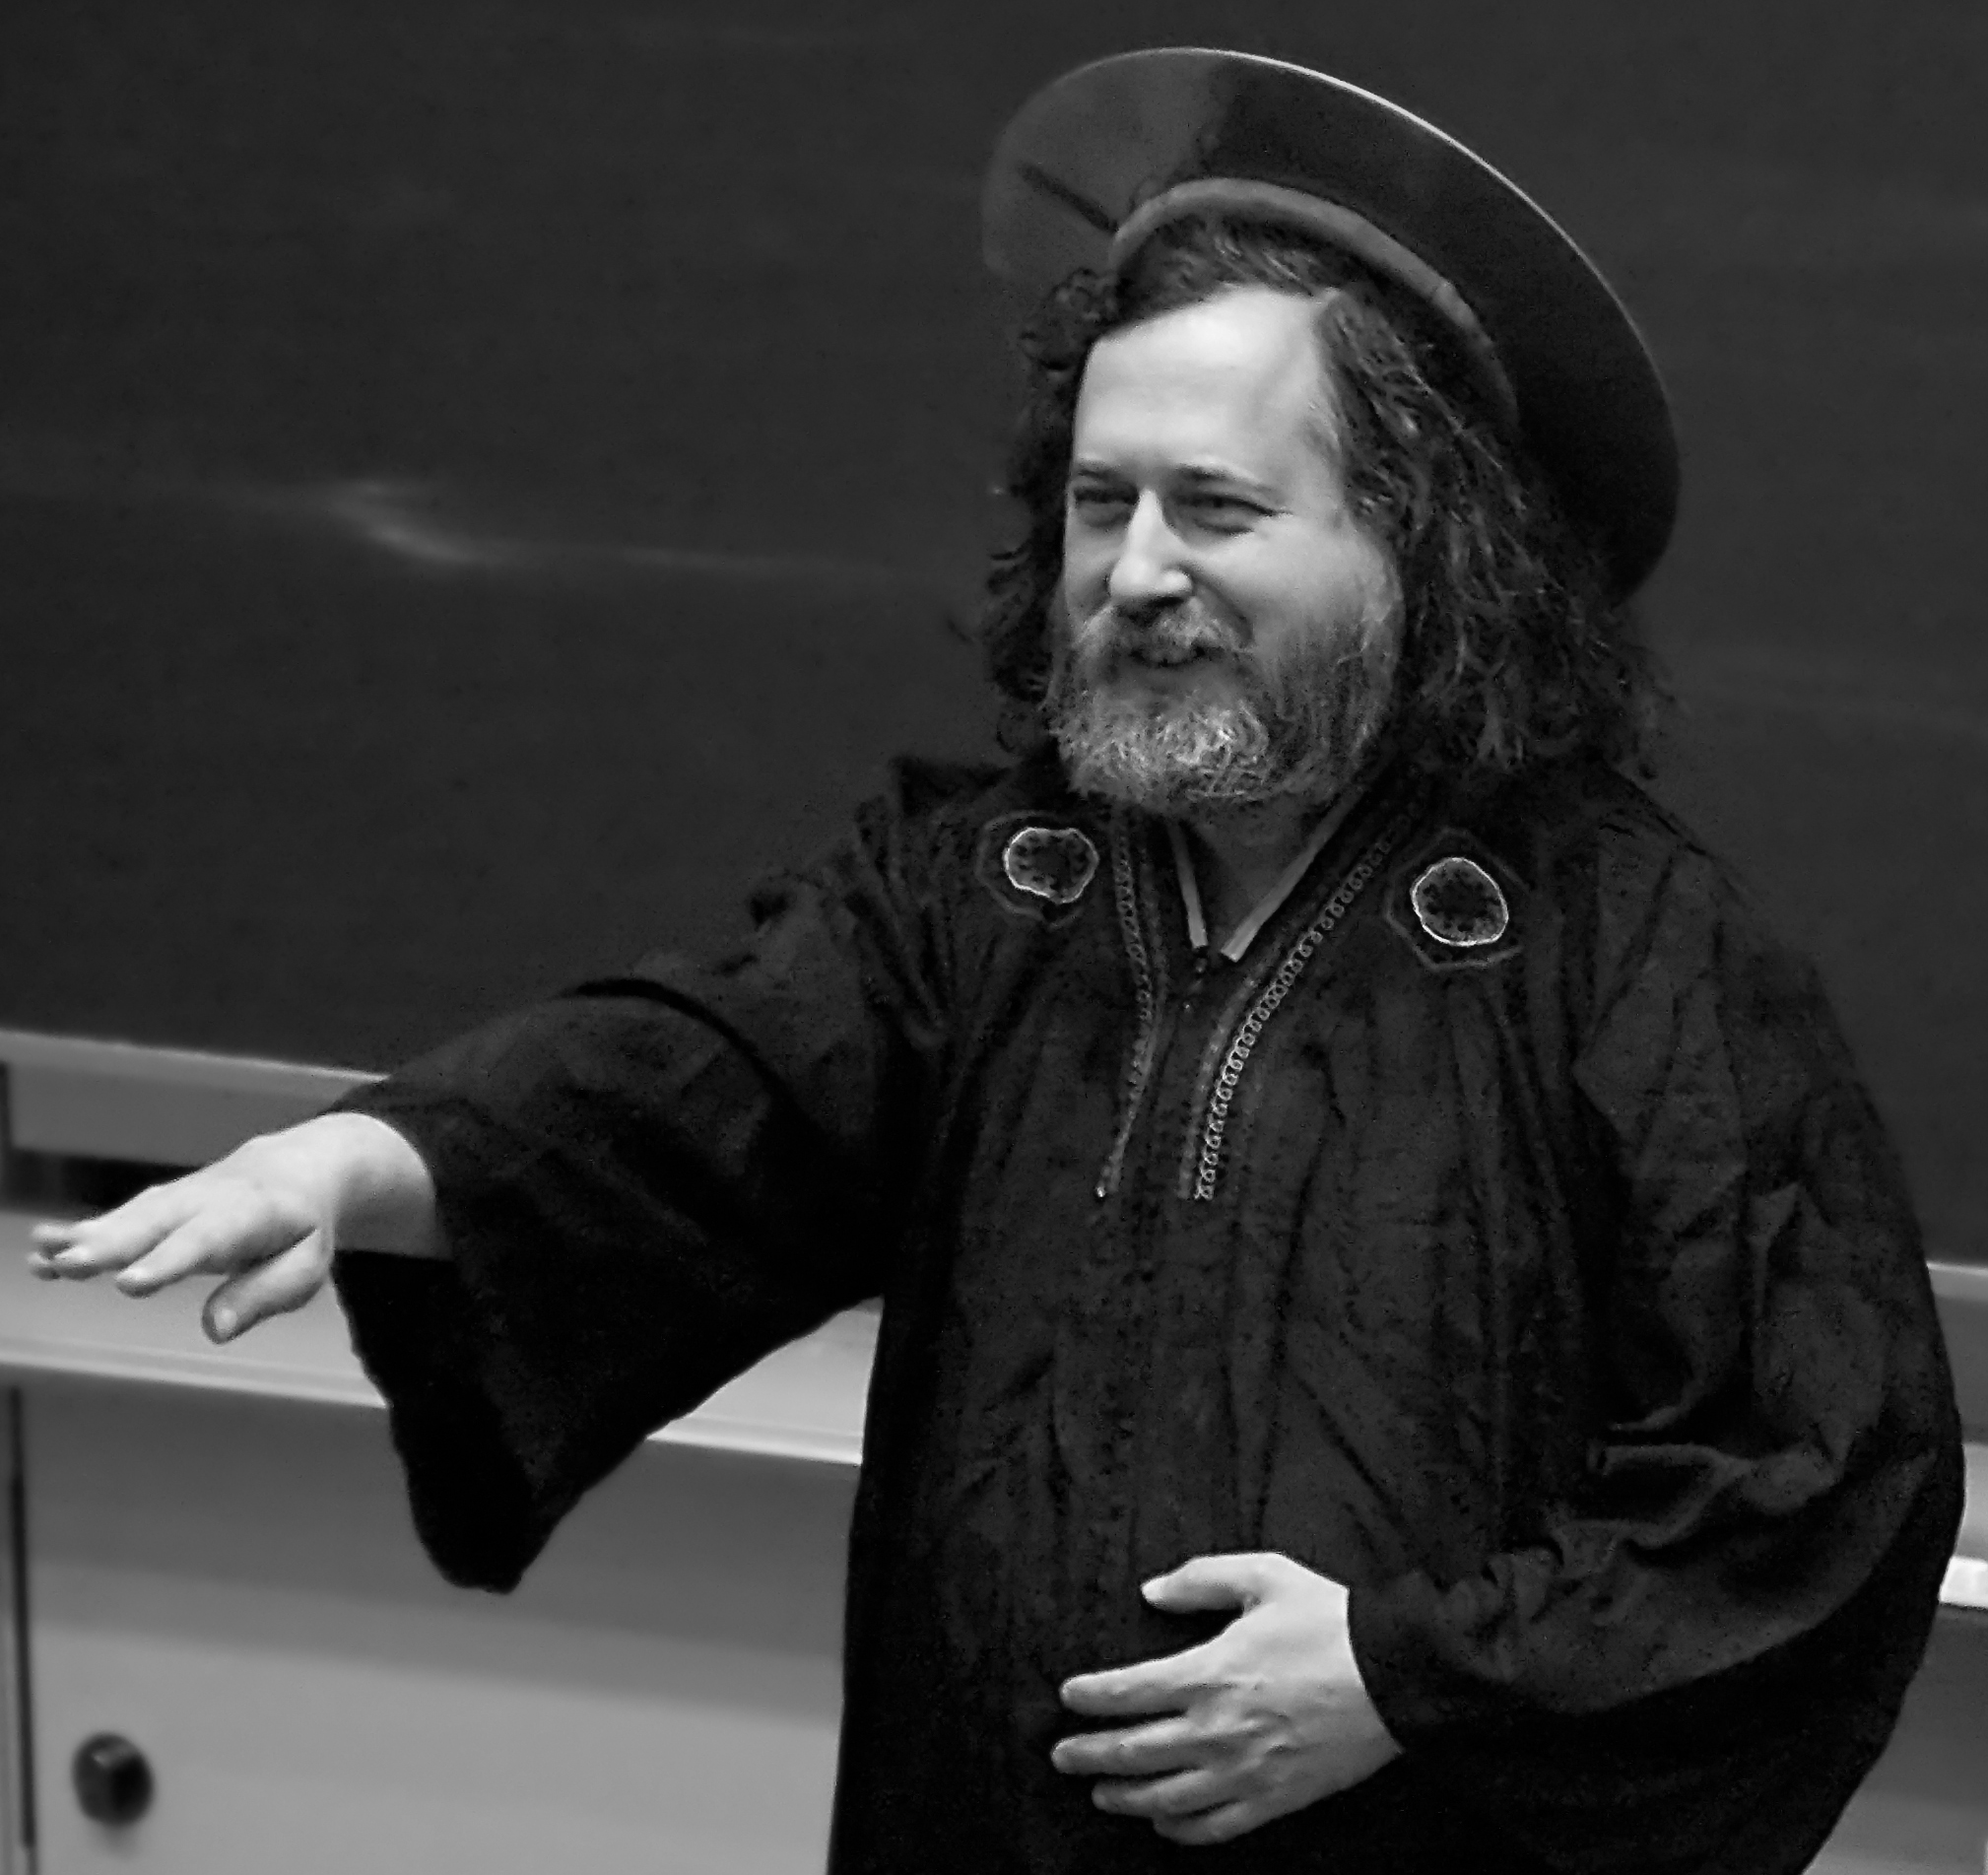
\includegraphics{stignucius}
  \caption{Stallman dressed as St. IGNUcius. The photo was taken by Stian Eikeland in Bergen, Norway on February 19, 2009.}
\end{figure}
\fi

\ifdefined\chs

\fi

\ifdefined\eng
The laughter turns into full-blown applause after a few seconds. As audience members clap, the computer disk on Stallman's head catches the glare of an overhead light, eliciting a perfect halo effect. In the blink of an eye, Stallman resembles a Russian religious icon.
\fi

\ifdefined\chs
大家的笑声在几秒钟之内变成了一阵掌声。大家在鼓掌的时候,理查德头上的那个硬盘碟片反射来一道强光,一下看起来,好像理查德头上真的顶了个光环。他眨了眨眼睛,又让我觉得他好似宗教领袖。
\fi

\ifdefined\eng
``Emacs was initially a text editor,'' says Stallman, explaining the getup. ``Eventually it became a way of life for many and a religion for some. We call this religion the Church of Emacs.''
\fi

\ifdefined\chs
理查德接着解释道:``Emacs最开始是一个编辑器,之后,很多人把它当作一种生活方式,还有一部分人把它作为一种信仰。我们把他们称作Emacs信徒。''
\fi

\ifdefined\eng
The skit is a lighthearted moment of self-parody, a humorous return-jab at the many people who might see Stallman's form of software asceticism as religious fanaticism in disguise. It is also the sound of the other shoe dropping -- loudly. It's as if, in donning his robe and halo, Stallman is finally letting listeners off the hook, saying, ``It's OK to laugh. I know I'm weird.''  [RMS: To laugh at someone for being weird is boorish, and it is not my intention to excuse that.  But I hope people will laugh at my St. IGNUcius comedy routine.]
\fi

\ifdefined\chs
很多人以为理查德对于自由软件一直都是不苟言笑,好像一个禁欲主义者一样。眼下这个玩笑倒是很好地否认了这种认识。在黑袍和光环之下,理查德好似在说:``你们尽情笑吧,我知道我这样很搞怪。''[理查德注:嘲笑别人行为怪异是不礼貌的,我并不鼓励这种做法。不过我是希望大家看到我圣·IGNUcius的扮相,能够笑起来]
\fi

\ifdefined\eng
Discussing the St. IGNUcius persona afterward, Stallman says he first came up with it in 1996, long after the creation of Emacs but well before the emergence of the ``open source'' term and the struggle for hacker-community leadership that precipitated it. At the time, Stallman says, he wanted a way to ``poke fun at himself,'' to remind listeners that, though stubborn, Stallman was not the fanatic some made him out to be. It was only later, Stallman adds, that others seized the persona as a convenient way to play up his reputation as software ideologue, as Eric Raymond did in an 1999 interview with the Linux.com web site:
\fi

\ifdefined\chs
之后和理查德聊起圣·IGNUcius这个舞台形象,他说他最早是在1996年开始在演讲中有这么个安排的。那会他早就开发了Emacs编辑器,那时也还没有``开源''这个词。理查德说,他当时希望能有个方式,能够``自娱自乐''一下;同时,也能告诉听众,理查德虽然固执,但还不至于疯狂到不苟言笑。不过这之后,理查德说,一些人借着这个舞台形象,把理查德形容为一个软件界的空想家。艾瑞克·雷蒙德就在1999年的一次与Linux.com的采访中,说道:
\fi

\ifdefined\eng
\begin{quote}
When I say RMS calibrates what he does, I'm not belittling or accusing him of insincerity. I'm saying that like all good communicators he's got a theatrical streak. Sometimes it's conscious -- have you ever seen him in his St. IGNUcius drag, blessing software with a disk platter on his head? Mostly it's unconscious; he's just learned the degree of irritating stimulus that works, that holds attention without (usually) freaking people out.\endnote{See ``Guest Interview: Eric S. Raymond,'' \textit{Linux.com} (May 18, 1999), \url{http://www.linux.com/interviews/19990518/8/}.}
\end{quote}
\fi

\ifdefined\chs
\begin{quote}
我说过,RMS(理查德·M·斯托曼名字的缩写)很会算计。我并不是说他不诚实,也不是说他虚情假意。我的意思是,他和很多布道者一样,非常有舞台感。有时候,他的这种行为是有意识的——你看过他扮成圣·IGNUcius的样子吗?他身穿黑袍,把一个碟片放在头顶。还有很多时候,那是无意识的行为。他很会掌握分寸,既能让你想去反驳,又不至于把人们吓跑\endnote{...........}。
\end{quote}
\fi

\ifdefined\eng
Stallman takes issue with the Raymond analysis. ``It's simply my way of making fun of myself,'' he says. ``The fact that others see it as anything more than that is a reflection of their agenda, not mine.''
\fi

\ifdefined\chs
理查德显然不同意艾瑞克·雷蒙德的说法。他说:``这不过是我自娱自乐罢了。谁要是从中还看到了别的东西,那只能说他们想多了。那都是他们脑子里的想法,不是我的。''
\fi

\ifdefined\eng
That said, Stallman does admit to being a ham. ``Are you kidding?'' he says at one point. ``I love being the center of attention.'' To facilitate that process, Stallman says he once enrolled in Toastmasters, an organization that helps members bolster their public-speaking skills and one Stallman recommends highly to others. He possesses a stage presence that would be the envy of most theatrical performers and feels a link to vaudevillians of years past. A few days after the Maui High Performance Computing Center speech, I allude to the 1999 LinuxWorld performance and ask Stallman if he has a Groucho Marx complex -- i.e., the unwillingness to belong to any club that would have him as a member.\endnote{RMS: Williams misinterprets Groucho's famous remark by treating it as psychological.  It was intended as a jab at the overt antisemitism of many clubs, which was why they would refuse him as a member.  I did not understand this either until my mother explained it to me.  Williams and I grew up when bigotry had gone underground, and there was no need to veil criticism of bigotry in humor as Groucho did.} Stallman's response is immediate: ``No, but I admire Groucho Marx in a lot of ways and certainly have been in some things I say inspired by him. But then I've also been inspired in some ways by Harpo.''
\fi

\ifdefined\chs
理查德也承认,他的这个表演有做作的成分。``就是开个玩笑。我很享受被万众瞩目。''他如是辩解。为了让自己的演讲技能可以更加娴熟,他甚至还加入过Toastermasters。这个社团旨在帮助人们提高演讲技能。理查德也曾向别人建议过Toastermasters。他加入了这个社团,逐渐掌握了一些舞台技巧。在这次茂宜高性能计算中心的演讲之后几天,我和理查德聊天的时候,问起他是否有种所谓的``格鲁桥·马克思情结''——就是像著名喜剧演员格鲁桥·马克思(Groucho Marx)所说的那样,拒绝加入任何希望收留他的俱乐部\endnote{...........}。理查德立即回复道:``不,但是我在很多方面都很敬仰格鲁桥·马克思,我说过的很多话都曾受到过他的启发。不过我也受到过汉普·马克思(Harpo Marx)的启发。''
\fi

\ifdefined\eng
The Groucho Marx influence is certainly evident in Stallman's lifelong fondness for punning. Then again, punning and wordplay are common hacker traits. Perhaps the most Groucho-like aspect of Stallman's personality, however, is the deadpan manner in which the puns are delivered. Most come so stealthily -- without even the hint of a raised eyebrow or upturned smile -- you almost have to wonder if Stallman's laughing at his audience more than the audience is laughing at him.
\fi

\ifdefined\chs
理查德一直以来对俏皮话,双关语的喜爱,恐怕的确是受了格鲁桥·马克思的影响。不过话说回来,双关语和文字游戏也从来都是黑客们的最爱。要说理查德真是有哪点会像格鲁桥,恐怕是他开玩笑之后,那副依旧淡定的表情。他的那些玩笑总是在不经意之间蹦出来,他自己则一脸严肃,眉毛都不抬。在你笑过之后,甚至反而会觉得理查德正在内心中笑话你。
\fi

\ifdefined\eng
Watching members of the Maui High Performance Computer Center laugh at the St. IGNUcius parody, such concerns evaporate. While not exactly a standup act, Stallman certainly possesses the chops to keep a roomful of engineers in stitches. ``To be a saint in the Church of Emacs does not require celibacy, but it does require making a commitment to living a life of moral purity,'' he tells the Maui audience. ``You must exorcise the evil proprietary operating systems from all your computers, and then install a wholly [holy] free operating system. And then you must install only free software on top of that. If you make this commitment and live by it, then you too will be a saint in the Church of Emacs, and you too may have a halo.''
\fi

\ifdefined\chs
不过你别担心,理查德可没笑话你。看到他在茂宜高性能计算中心演讲时候的圣·IGNUcius的扮相,你的顾虑就打消了。他这表演虽然不比单口相声,但理查德总还是有能耐把一屋子的工程师聚在一起。``Emacs教会之中,不必戒色禁欲。但也需你心存底线,道清德厚,有所顾忌。''理查德继续对听众说道:``你要在自己的电脑之上,趋邪扶正。专有软件,卸载删除。辟得净土,以敬用户。系统上下,软件自由。茫茫众生,守此信条,即入本会,得道称圣。对了,到时候你没准也能拿到这样一个光环。''
\fi

\ifdefined\eng
The St. IGNUcius skit ends with a brief inside joke. On most Unix systems and Unix-related offshoots, the primary competitor program to Emacs is vi, pronounced vee-eye, a text-editing program developed by former UC Berkeley student and current Sun Microsystems chief scientist, Bill Joy. Before doffing his ``halo,'' Stallman pokes fun at the rival program. ``People sometimes ask me if it is a sin in the Church of Emacs to use vi,'' he says. ``Using a free version of vi is not a sin; it is a penance. So happy hacking.''\endnote{The service of the Church of Emacs has developed further since 2001. Users can now join the Church by reciting the Confession of the Faith: ``There is no system but GNU, and Linux is one of its kernels.'' Stallman sometimes mentions the religious ceremony known as the Foobar Mitzvah, the Great Schism between various rival versions of Emacs, and the cult of the Virgin of Emacs (which refers to any person that has not yet learned to use Emacs).  In addition, ``vi vi vi'' has been identified as the Editor of the Beast.}
\fi

\ifdefined\chs
圣·IGNUcius的演出以一个圈内冷笑话做结尾。在大多数UNIX或者类UNIX系统上,和Emacs齐名的另外一款编辑器名为vi。vi编辑器最早是由比尔·乔伊(Bill Joy)开发。他当年是加州大学伯克利分校的学生,如今是Sun微系统公司的首席科学家。理查德在摘掉自己头顶的``光环''之前,给vi这个竞争对手开了个小玩笑。``人们会问,在Emacs教会中使用vi是否算作原罪。倘若使用的是自由版的vi,那不能称之为罪。可以算是自罚赎罪。那么,Happy Hacking!''\endnote{...........}
\fi

\ifdefined\eng
After a brief question-and-answer session, audience members gather around Stallman. A few ask for autographs. ``I'll sign this,'' says Stallman, holding up one woman's print out of the GNU General Public License, ``but only if you promise me to use the term GNU/Linux instead of Linux'' (when referring to the system), ``and tell all your friends to do likewise.''
\fi

\ifdefined\chs
一个简短的提问环节过后,听众们围在理查德周围,有些人向他索要签名。理查德拿着一位女士打印出来的GNU通用许可证,说:``我可以答应你在上面签名,不过你要答应我,在指代那整个操作系统的时候,使用GNU/Linux这个词。并且要告诉你的朋友也这么做。''
\fi

\ifdefined\eng
The comment merely confirms a private observation. Unlike other stage performers and political figures, Stallman has no ``off'' mode. Aside from the St. IGNUcius character, the ideologue you see onstage is the ideologue you meet backstage. Later that evening, during a dinner conversation in which a programmer mentions his affinity for ``open source'' programs, Stallman, between bites, upbraids his tablemate: ``You mean free software. That's the proper way to refer to it.''
\fi

\ifdefined\chs
他的这个举动倒是证实了我的想法。和演员,政客不同,理查德的行为会始终如一,不会切换到``台下模式''。在圣·IGNUcius这个角色中看到的那份理想主义,会一直体现在理查德的每个言行之上。在演讲之后的晚餐上,一位程序员向理查德提起了自己参与``开源''软件的经历,理查德还没顾得上咽下嘴里的食物,说道:``你是说自由软件吧。用自由软件这个词恐怕更恰当。''
\fi

\ifdefined\eng
During the question-and-answer session, Stallman admits to playing the pedagogue at times. ``There are many people who say, `Well, first let's invite people to join the community, and then let's teach them about freedom.' And that could be a reasonable strategy, but what we have is almost everybody's inviting people to join the community, and hardly anybody's teaching them about freedom once they come in.''
\fi

\ifdefined\chs
在演讲结束后的提问环节,理查德承认自己很多时候有些咬文嚼字。``很多人会劝我:`咱们先把人邀请进我们的圈子,然后再教会他们什么是自由。'这也许是个好策略,但是我们当下的情况是,基本所有人都在邀请朋友们进到这个圈子里,可却没有几个人会告诉朋友自由是什么。''
\fi

\ifdefined\eng
The result, Stallman says, is something akin to a third-world city. ``You have millions of people moving in and building shantytowns, but nobody's working on step two: getting them out of those shantytowns. If you think talking about software freedom is a good strategy, please join in doing step two. There are plenty working on step one. We need more people working on step two.''
\fi

\ifdefined\chs
最后的结果,用理查德的话说,就是好比很多第三世界国家建立的城市。``你把百万千万的人扔到城市中,结果是在城市里建起了成千上万的城中村,贫民窟。但是没人开始着手做下一步的工作:把城中村,贫民窟里的人解救出来。如果你觉得讨论软件用户的自由是有意义的,那么请加入我们,开始做第二步工作。很多人都在做第一步,但这第二步却无人问津。''
\fi

\ifdefined\eng
Working on ``step two'' means driving home the issue that freedom, not acceptance, is the root issue of the free software movement. Those who hope to reform the proprietary software industry from the inside are on a fool's errand. ``Change from the inside is risky,'' Stallman stays. ``Unless you're working at the level of a Gorbachev, you're going to be neutralized.''
\fi

\ifdefined\chs
这``第二步''工作直指自由软件运动的核心:自由软件的重点并非是装机量用户量,而是赋予用户自由。有些人希望能从内部瓦解整个专有软件工业,这实在是痴人梦话。理查德说:``从内部瓦解实在不现实,除非你能像当年戈尔巴乔夫那样攀到高位,否则你多半会被同化。''
\fi

\ifdefined\eng
Hands pop up. Stallman points to a member of the golf shirt-wearing contingent. ``Without patents, how would you suggest dealing with commercial espionage?''
\fi

\ifdefined\chs
又有很多人举手提问,理查德随机选择了一位身穿高尔夫衬衫的听众,这位听众问道:``如果没有专利,你会建议如何防止商业间谍?''
\fi

\ifdefined\eng
``Well, those two questions have nothing to do with each other, really,'' says Stallman.
\fi

\ifdefined\chs
理查德答:``嗯……这其实是两个互不相关的问题。''
\fi

\ifdefined\eng
``But I mean if someone wants to steal another company's piece of software.''
\fi

\ifdefined\chs
提问者补充道:``我是说,如果有人想要窃取另一个公司的软件。''
\fi

\ifdefined\eng
Stallman's recoils as if hit by a poisonous spray. ``Wait a second,'' Stallman says. ``Steal? I'm sorry, there's so much prejudice in that statement that the only thing I can say is that I reject that prejudice.'' Then he turns to the substance of the question. ``Companies that develop nonfree software and other things keep lots and lots of trade secrets, and so that's not really likely to change. In the old days -- even in the 1980s -- for the most part programmers were not aware that there were even software patents and were paying no attention to them. What happened was that people published the interesting ideas, and if they were not in the free software movement, they kept secret the little details. And now they patent those broad ideas and keep secret the little details. So as far as what you're describing, patents really make no difference to it one way or another.''
\fi

\ifdefined\chs
理查德立即反应道:``等等,你说`窃取'?不好意思,你的这番陈述里包含太多偏见了。我只能说,我很难认同这些偏见。''接着,理查德转向问题本身:``各个公司,它们可能会开发专有软件,或者开发任何别的东西。无论开发什么,多少都会有些商业机密,它们无论如何都会保守这些机密。这个事实恐怕很难改变。在早年间——哪怕到了八十年代——绝大部分程序员都没想到过把软件去申请专利。人们会发表文章记录自己有趣的想法,如果他们不认同自由软件的理念,他们可能会在文章中甚少提及各种细节。如今,他们同样写篇文章,笼统地记录下那些想法,依然保守着各种细节。如今不同的是,他们把这文章拿去专利局,就可以申请下专利。软件专利并没能把这个事实改变多少。''
\fi

\ifdefined\eng
``But if it doesn't affect their publication,'' a new audience member jumps in, his voice trailing off almost as soon as he starts speaking.
\fi

\ifdefined\chs
``但如果不会影响他们公开发表的文章……''另一位听众起立发言,但还没说完,就被打断了。
\fi

\ifdefined\eng
``But it does,'' Stallman says. ``Their publication is telling you that this is an idea that's off limits to the rest of the community for 20 years. And what the hell good is that? Besides, they've written it in such a hard way to read, both to obfuscate the idea and to make the patent as broad as possible, that it's basically useless looking at the published information [in the patent] to learn anything anyway. The only reason to look at patents is to see the bad news of what you can't do.''
\fi

\ifdefined\chs
``但它的确影响了。''理查德说:``在版权局能查到的公开文章就是告诉你,从现在开始往后20年,这个想法任何人都不能随便用。这能算是什么好处吗?还请注意,他们在文章中,会把想法描述得像天书一般难懂,而且会尽量把话说得模棱两可,这样就可以让这版权覆盖尽可能多的地方。没有几个人会从那些文章里去学习哪个版权所保护的技术。你能从那些文章中了解到的信息,只能告诉你什么技术你不能用。''
\fi

\ifdefined\eng
The audience falls silent. The speech, which began at 3:15, is now nearing the 5:00 whistle, and most listeners are already squirming in their seats, antsy to get a jump start on the weekend. Sensing the fatigue, Stallman glances around the room and hastily shuts things down. ``So it looks like we're done,'' he says, following the observation with an auctioneer's ``going, going, gone'' to flush out any last-minute questioners. When nobody throws their hand up, Stallman signs off with a traditional exit line.
\fi

\ifdefined\chs
听众一时安静下来。这个演讲从下午3:15开始,现在已经将近五点。下面很多听众已经有些坐不住了。理查德也察觉到了听众的倦意,他目光扫视了全场,说道:``那么,今天就到这儿吧。''他又停顿了一下,等到确认没有人有问题之后,理查德又重复了一遍那句口头语:
\fi

\ifdefined\eng
``Happy hacking,'' he says.
\fi

\ifdefined\chs
``Happy Hacking。''理查德说。
\fi

\theendnotes
\setcounter{endnote}{0}
